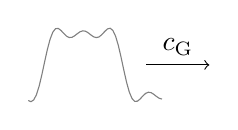
\begin{tikzpicture}[scale=1, domain=-0.2:1.5, samples=50]
\draw[gray] plot (\x,{0.5*sin(\x*180)+(0.5/3)*sin(\x*180*3)+(0.5/5)*sin(\x*180*5))});
\draw[->] (1.3, 0) -- node[above] {$c_\mathrm{G}$} (2.1, 0);
\end{tikzpicture}
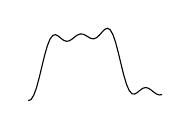
\begin{tikzpicture}[scale=1, domain=-0.2:1.5, samples=50]
\draw plot (\x,{0.45*sin(\x*180)+(0.45/3)*sin(\x*180*3+15)+(0.45/5)*sin(\x*180*5+30))});
\end{tikzpicture}
